\documentclass[12pt]{scrartcl}

\usepackage{libertine, libertinust1math}
\usepackage[T1]{fontenc}

\usepackage{tikz}
\usepackage{drawstack}
\usepackage{listings}
\usepackage{enumitem}

\usepackage{lastpage}
\usepackage{fancyhdr}

\usepackage[hidelinks]{hyperref}

\usepackage{caption}

\pagestyle{fancy}
\fancyfoot{}

\rhead{Prova Finale (Progetto di Reti Logiche)}
\chead{}
\lfoot{}
\rfoot{Pagina \thepage\ di \pageref{LastPage}}
\renewcommand{\headrulewidth}{0.4pt}
\renewcommand{\footrulewidth}{0.4pt}

\usetikzlibrary{arrows}
\usetikzlibrary{calc, arrows.meta}
\usetikzlibrary{positioning, decorations.pathreplacing}
\usetikzlibrary{automata}
\usetikzlibrary{matrix}

\renewcommand{\figurename}{Figura}
\renewcommand{\tablename}{Tabella}

\newcommand{\specialcell}[2][l]{%
	\begin{tabular}[#1]{@{}l@{}}#2\end{tabular}
}

\setlist[itemize,1]{label={\Large\textbullet}}
\setlist[0]{itemsep=2pt}

%opening
\title{Prova Finale (Progetto di Reti Logiche)}
\subtitle{Docente: Fabio Salice - A.A. 2019/2020}

% a cura di
\author{Samuele Negrini (Codice Persona 10539341 - Matricola 866797)}
\date{}


\begin{document}
	\thispagestyle{empty}
	\maketitle
	
	\renewcommand{\contentsname}{Indice}
	\tableofcontents
	
	\section{Introduzione}
La specifica della Prova Finale (Progetto di Reti Logiche) 2019 è ispirata al metodo di codifica a bassa dissipazione di potenza denominato \textit{Working Zone}.\newline
Tale metodo è pensato per il Bus Indirizzi e si usa per trasformare il valore di un indirizzo, quando questo viene trasmesso, se appartiene a certi intervalli (detti appunto working-zone). Una working-zone è definita come un intervallo di indirizzi di dimensione fissa ($D_{wz}$) che parte da un indirizzo base. All'interno dello schema di codifica possono esistere multiple working-zone ($N_{wz}$).

\subsection{Obiettivo del progetto}
Dati gli indirizzi base delle working-zone e l'indirizzo da codificare, si vuole implementare un componente hardware descritto in VHDL in grado di leggere l'indirizzo da codificare e gli indirizzi base delle working-zone, verificare l'appartenenza dell'indirizzo da codificare a tali working-zone e produrre l'indirizzo opportunamente codificato in uscita.
In pratica, il modulo da sviluppare si comporta come un \textbf{encoder} di indirizzi.

\subsection{Specifica generale}
Si consideri l'indirizzo da trasmettere $ADDR$. Lo schema di codifica implementato è il seguente:
\begin{itemize}
	\item se $ADDR$ non appartiene a nessuna Working Zone \textbf{[WZ MISS]}, verrà trasmesso un bit addizionale ${WZ}_{BIT}=0$ concatenato ad $ADDR$ (${WZ}_{BIT}$ \& $ADDR$, dove \& è il simbolo di concatenazione);
	
		\begin{figure}[!htb]
			\tikzstyle{int}=[draw, fill=black!10, minimum size=4em]
\tikzstyle{init} = [pin edge={to-,thin,black}]

\centering

\begin{tikzpicture}[node distance=6cm,auto,>=latex']
\node [int] (a) {ENCODER};
\node (b) [left of=a,node distance=5cm]{SOURCE};
\node (end) [right of=a, node distance=8cm]{DEST};
\path[->] (b) edge node {$ADDR$} (a);
\draw[->] (a) edge node {$0$ \& $ADDR$} (end);
\end{tikzpicture}
			\caption{codifica di un indirizzo non appartenente a nessuna WZ.}
			\label{fig:addr_no_wz}
		\end{figure}

	\item se $ADDR$ appartiene ad una Working Zone \textbf{[WZ HIT]}, verrà trasmesso ${WZ}_{BIT}=1$ concatenato a due valori ${WZ}_{NUM}$ e ${WZ}_{OFFSET}$, rappresentanti rispettivamente:
	\begin{itemize}
		\item il numero della working-zone al quale l'indirizzo appartiene, codificato in binario;
		
		\item l'offset rispetto all'indirizzo di base della working-zone, codificato come one-hot.
	\end{itemize}

	
	
	\begin{figure}[!htb]
		\tikzstyle{int}=[draw, fill=black!10, minimum size=4em]
\tikzstyle{init} = [pin edge={to-,thin,black}]

\centering

\begin{tikzpicture}[node distance=6cm,auto,>=latex']
    \node [int] (a) {ENCODER};
    \node (b) [left of=a,node distance=5cm]{SOURCE};
    \node (end) [right of=a, node distance=8cm]{DEST};
    \path[->] (b) edge node {$ADDR$} (a);
    \draw[->] (a) edge node {$1$ \& ${WZ}_{NUM}$ \& ${WZ}_{OFFSET}$} (end);
\end{tikzpicture}	
		\caption{codifica di un indirizzo appartenente ad una WZ.}
		\label{fig:addr_in_wz}
	\end{figure}
\end{itemize}

Si considerino 7 bit per l'indirizzo da codificare (quindi indirizzi validi da 0 a 127).\newline
Il numero di working-zone è 8 ($N_{wz}=8$) mentre la dimensione della working-zone è di 4 indirizzi incluso quello base ($D_{wz}=4$). Questo comporta che l'indirizzo codificato sarà composto da 8 bit: 1 bit per ${WZ}_{BIT}$ + 7 bit per $ADDR$, oppure 1 bit per ${WZ}_{BIT}$, 3 bit per codificare in binario a quale tra le 8 working-zone l'indirizzo appartiene, e 4 bit per codificare one-hot il valore dell'offset di $ADDR$ rispetto all'indirizzo base.\newline

\textbf{Esempio}: codifica di $ADDR$=33, sapendo che la WZ 3 ha come indirizzo di base 31.
\begin{figure}[!htb]
	\centering
	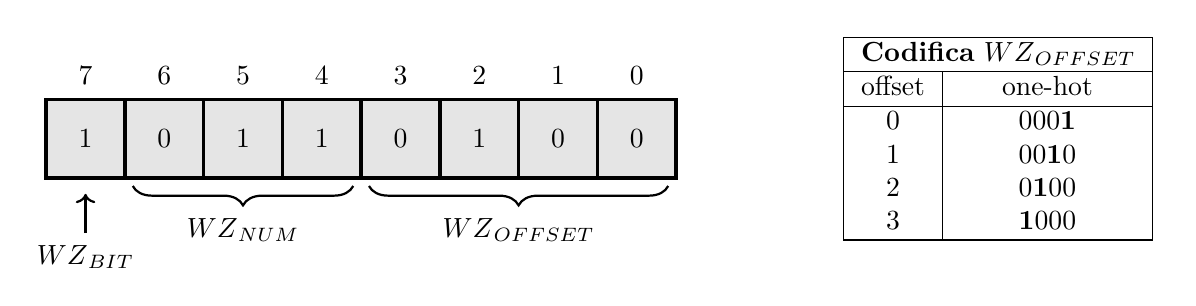
\begin{tikzpicture}[box/.style={fill=black!10, rectangle,draw=black, very thick, minimum size=1cm}]
	
	\foreach \i in {0,...,7} {
		\node at (8-\i-1,0.8){\i};
	}
	
	\foreach \y [count=\x] in {1,0,1,1,0,1,0,0} {
		\node[box] at (\x-1,0){\y};
	}

	\draw[decorate,decoration={brace, amplitude=7pt, raise=0pt, mirror}, thick] (0.6,-.6) -- node[below=8pt]{${WZ}_{NUM}$} (3.4,-.6);
	\draw[decorate,decoration={brace, amplitude=7pt, raise=0pt, mirror}, thick] (3.6,-.6) -- node[below=8pt]{${WZ}_{OFFSET}$} (7.4,-.6);
	\draw[->, thick] (0,-1.2) --  node[below=2pt,yshift=-2mm]{${WZ}_{BIT}$} (0,-.7);

	\node[text width=4cm, anchor=west, right] at (9.5,0) {	
		\begin{tabular}{ |c|c| }
		\hline
		\multicolumn{2}{|c|}{\textbf{Codifica ${WZ}_{OFFSET}$}} \\
		\hline
		offset & one-hot\\
		\hline
		0 & 000\textbf{1}\\
		1 & 00\textbf{1}0\\
		2 & 0\textbf{1}00\\
		3 & \textbf{1}000\\
		\hline
		\end{tabular}
	};
\end{tikzpicture}

	\caption{ADDR appartiene alla WZ 3, con offset 2 (in one-hot).}
	\label{fig:es_addr_in_wz}
\end{figure}



\subsection{Interfaccia del componente}
Il componente descritto possiede la seguente interfaccia:

\begin{lstlisting}[basicstyle=\small, language=VHDL]
entity project_reti_logiche is
port (
	i_clk 		: in std_logic;
	i_start 	: in std_logic;
	i_rst 		: in std_logic;
	i_data 		: in std_logic_vector(7 downto 0);
	o_address 	: out std_logic_vector(15 downto 0);
	o_done 		: out std_logic;
	o_en 		: out std_logic;
	o_we 		: out std_logic;
	o_data 		: out std_logic_vector(7 downto 0)
);
end project_reti_logiche;
\end{lstlisting}


In particolare:
\begin{itemize}
	\item \lstinline[columns=fixed]{i_clk} è il segnale di \lstinline[columns=fixed]{CLOCK} in ingresso generato dal Test Bench;
	
	\item \lstinline[columns=fixed]{i_start} è il segnale di \lstinline[columns=fixed]{START} generato dal Test Bench;
	
	\item \lstinline[columns=fixed]{i_rst} è il segnale di \lstinline[columns=fixed]{RESET} che inizializza la macchina pronta per ricevere il primo segnale di \lstinline[columns=fixed]{START};
	
	\item \lstinline[columns=fixed]{i_data} è il segnale (vettore) che arriva dalla memoria in seguito ad una richiesta di lettura;
	
	\item \lstinline[columns=fixed]{o_address} è il segnale (vettore) di uscita che manda l'indirizzo alla memoria;
	
	\item \lstinline[columns=fixed]{o_done} è il segnale di uscita che comunica la fine dell'elaborazione e il dato di uscita scritto in memoria;
	
	\item \lstinline[columns=fixed]{o_en} è il segnale di \lstinline[columns=fixed]{ENABLE} da dover mandare alla memoria per poter comunicare (sia in lettura che in scrittura);
	
	\item \lstinline[columns=fixed]{o_we} è il segnale di \lstinline[columns=fixed]{WRITE ENABLE} da dover mandare alla memoria (=1) per poter scriverci. Per leggere da memoria esso deve essere 0;
	
	\item \lstinline[columns=fixed]{o_data} è il segnale (vettore) di uscita dal componente verso la memoria.
\end{itemize}

\subsection{Dati e memoria}
Il componente dovrà gestire la comunicazione con una memoria ausiliaria sulla quale saranno presenti i dati in ingresso e andranno salvati quelli in uscita.\newline
I dati, ciascuno di dimensione 8 bit, sono memorizzati sulla memoria con indirizzamento al Byte partendo dalla posizione 0.
Anche l'indirizzo da codificare che è da specifica di 7 bit viene memorizzato su 8 bit (il valore dell'ottavo bit sarà sempre zero).

La memoria è così organizzata:
\begin{itemize}
	\item Le posizioni da 0 a 7 sono usate per memorizzare gli otto indirizzi base delle working-zone;
	
	\item La posizione 8 è usata per memorizzare il valore (indirizzo) da codificare ($ADDR$);
	
	\item La posizione 9 è usata per scrivere il valore codificato in uscita.
\end{itemize}

\begin{figure}[!htb]
	\centering
	\tikzstyle{freecell}=[fill=black!10]
\tikzstyle{occupiedcell}=[fill=black!10]

\renewcommand{\llcell}[3]{
	\addtocounter{cellnb}{-#1}
	\setcounter{ptrnb}{0}
	\draw[#2] (0,\value{cellnb}) +(-2.8,-.5) rectangle +(2.8,-.5+#1);
	\draw (0,\value{cellnb}+#1/2-0.5)  node(currentcell) {#3};
}

\renewcommand{\finishframe}[1]{
	\draw[snake=brace, line width=0.6pt, segment amplitude=8pt]
	(-2.8,\value{cellnb}-0.5) -- (-2.8,\value{startframe}-0.5);
	\draw (-5.4cm,\value{cellnb}*0.5+\value{startframe}*0.5-0.7) node
	{\parbox{3cm}{%
	\begin{flushright}
		#1
	\end{flushright}}};
}

\renewcommand{\separator}[1][freecell,very thick]{
	\draw[#1] (0,\value{cellnb}) +(-2.8,-.5) -- +(2.8,-.5);
}

\renewcommand{\cellcom}[1]{
	\draw (3.1,\value{ptrnb}*0.5+\value{cellnb}) node[anchor=west] {#1};
	\addtocounter{ptrnb}{1}
}

\renewcommand{\stackbottom}[1][freecell]{
	\addtocounter{cellnb}{-1}
	\draw[#1] (0,\value{cellnb})
	+(-2.8,-.5) -- +(-2.8,+.5) -- +(2.8,+.5) -- +(2.8,-.5);
	\draw (0,\value{cellnb}) node{...};
}


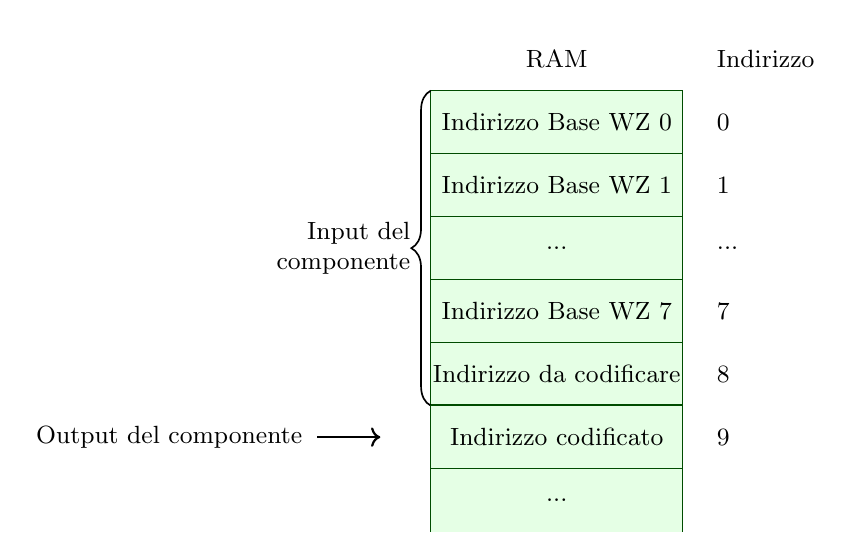
\begin{tikzpicture}[scale=0.8]
	\small
	\cell[draw=none]{RAM} \cellcom{Indirizzo}
	\startframe
	\cell{Indirizzo Base WZ 0}        \cellcom{0}
	\cell{Indirizzo Base WZ 1}        \cellcom{1}
	\cell{...} \cellcom{...}
	\cell{Indirizzo Base WZ 7} \cellcom{7}
	\cell{Indirizzo da codificare}     \cellcom{8}
	\finishframe{Input del componente}
	\separator
	\cell{Indirizzo codificato} \cellcom{9}
	\stackbottom{}
	
	\draw[->, thick] (-3.8,-7) --  node[left=2pt,xshift=-4mm]{Output del componente} (-2.8,-7);
	
\end{tikzpicture}

	\caption{indirizzi della RAM rilevanti.}
	\label{fig:ram_1}
\end{figure}

% %% stack-example.tex
  %% Copyright 2010 Matthieu Moy <Matthieu.Moy@imag.fr>
  %
  % This work may be distributed and/or modified under the
  % conditions of the LaTeX Project Public License, either version 1.3
  % of this license or (at your option) any later version.
  % The latest version of this license is in
  %   http://www.latex-project.org/lppl.txt
  % and version 1.3 or later is part of all distributions of LaTeX
  % version 2005/12/01 or later.
  %
  % This work has the LPPL maintenance status `maintained'.
  %
  % The Current Maintainer of this work is M. Matthieu Moy.
  %
  % This work consists of the files drawstack.sty and the example file
  % stack-example.tex.

\documentclass{article}

\usepackage{drawstack}

% Use this instead if you don't want colors.
% \usepackage[nocolor]{drawstack}

\title{{\tt drawstack.sty}: Draw execution stack easily in LaTeX}
\author{Matthieu Moy}

\begin{document}
\maketitle

{\tt drawstack} is a LaTeX package to easily draw execution stack
(typically to illustrate assembly language notions), written on top of
TikZ. This file serves as an example of usage of {\tt drawstack}, and
serves as documentation for this package. Read the source code and
comments to see how to use it.

\section{Minimalistic example}

% The main feature of the package is to define an environment
% drawstack.
\begin{drawstack}
  % Within the environment, draw stack elements with \cell{...}
  \cell{First cell}
  \cell{Second cell}
\end{drawstack}

\section{Grouping cells into stack frames}

\begin{drawstack}
  \startframe
  \cell{First cell}
  \cell{Second cell}
  \finishframe{Some stack frame}
  \cell{Not interesting}
  \startframe
  \cell{Next stack frame}
  \cell{Next stack frame}
  \finishframe{Another stack frame}
\end{drawstack}

\section{Stack and Base pointers}

\begin{drawstack}
  \startframe
  % \cellcom writes something on the right-hand side of a cell.
  \cell{loc2} \cellcom{-8(\%ebp)}
  \cell{loc1} \cellcom{-4(\%ebp)}
  % \esp and \ebp are stack pointer and base pointer in Pentium.
  % These macros are simple shortcuts for \cellptr{...}
  \cell{Sauvegarde \%ebp} \esp \ebp
  \cell{@ retour} \cellcom{4(\%ebp)}
  \finishframe{fonction\\ {\tt f}}
  \startframe
  \cell{} \cellcom{8(\%ebp)}
  \cell{}
  \finishframe{fonction\\ {\tt main}}
\end{drawstack}

\section{Padding}

\begin{drawstack}
  \cell{above padding}
  \padding{3}{nothing here}
  \cell{below padding}
\end{drawstack}

\section{Below/Above stack pointer}

\begin{drawstack}
  \cell{Top}
  \cell{Below top}
  % \bcell is just like \cell, but in a different color.
  \bcell{Above bottom} \cellptr{Stack pointer here}
  \bcell{Bottom}
\end{drawstack}

\section{Highlighting some cell}

\begin{drawstack}
  \cell{Uninteresting cell}
  \cell{Interesting cell} \cellround{Yes, this one!}
\end{drawstack}

\section{Structures without a stack structure}

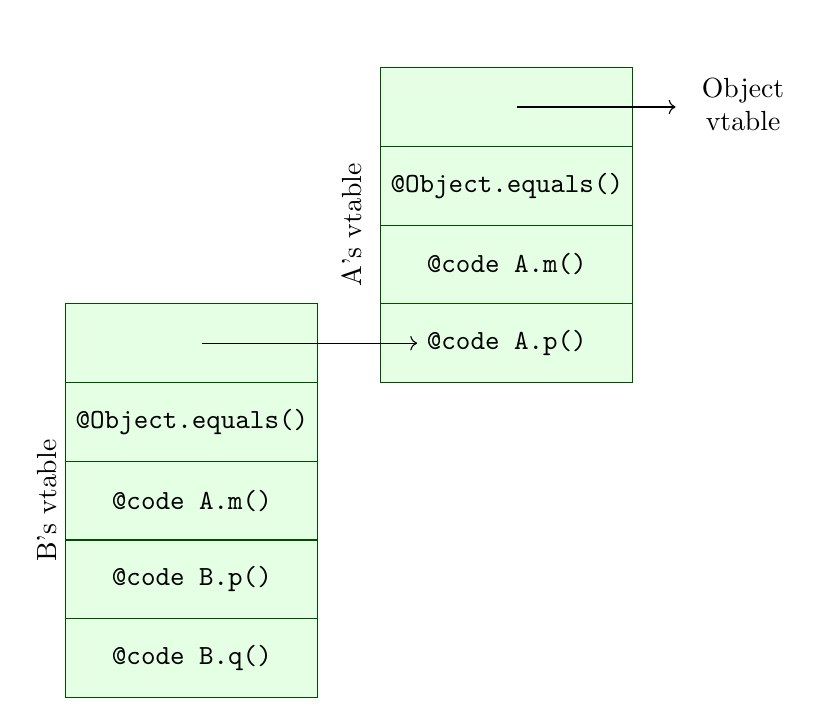
\begin{tikzpicture}
  \draw (3, -1) node (Otm) {
    \begin{tabular}{c}
      Object\\vtable
    \end{tabular}
  };

  \drawstruct{(0,0)}
  \structcell[freecell]{~} \coordinate (Atm) at (currentcell.east);
  \structcell[freecell]{\texttt{@Object.equals()}}
  \structcell[freecell]{\texttt{@code A.m()}}
  \structcell[freecell]{\texttt{@code A.p()}} \coordinate (A) at (currentcell.west);
  \structname{
    \begin{tabular}{c}
      A's vtable
    \end{tabular}
  }

  \drawstruct{(-4,-3)}
  \structcell[freecell]{} \coordinate (Btm) at (currentcell.east);
  \structcell[freecell]{\texttt{@Object.equals()}}
  \structcell[freecell]{\texttt{@code A.m()}}
  \structcell[freecell]{\texttt{@code B.p()}}
  \structcell[freecell]{\texttt{@code B.q()}}
  \structname{B's vtable}

  \draw[->] (Btm) -- (A);
  \draw[->] (Atm) -- (Otm);
\end{tikzpicture}

\section{Structures and stack together}

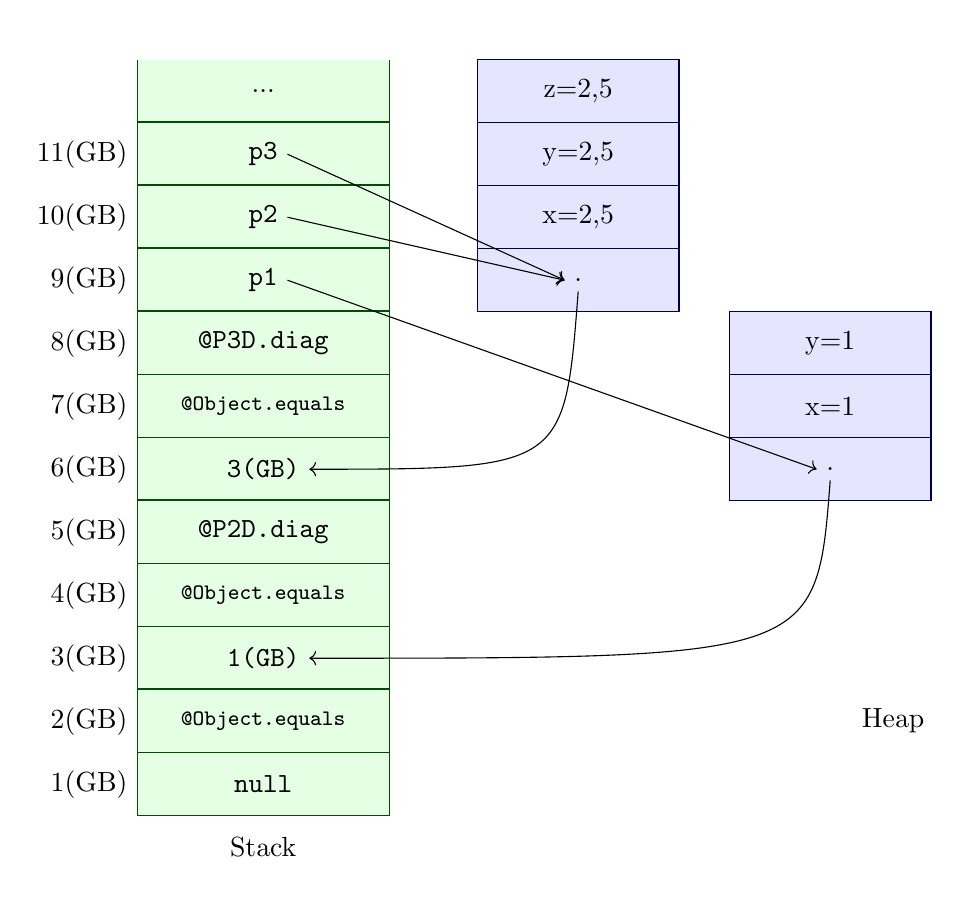
\begin{tikzpicture}[scale=.8]

  \stacktop{}
  \separator
  \cell{\texttt{p3}}        \cellcomL{11(GB)} \coordinate (p3) at (currentcell.east);
  \separator
  \cell{\texttt{p2}}        \cellcomL{10(GB)} \coordinate (p2) at (currentcell.east);
  \separator
  \cell{\texttt{p1}}        \cellcomL{ 9(GB)} \coordinate (p1) at (currentcell.east);
  \separator
  \cell{\texttt{@P3D.diag}} \cellcomL{ 8(GB)}
  \cell{\texttt{\footnotesize @Object.equals}} \cellcomL{ 7(GB)}
  \cell{\texttt{3(GB)}}     \cellcomL{ 6(GB)} \coordinate (T1) at (currentcell.east);
  \separator
  \cell{\texttt{@P2D.diag}} \cellcomL{ 5(GB)}
  \cell{\texttt{\footnotesize @Object.equals}} \cellcomL{ 4(GB)}
  \cell{\texttt{1(GB)}}     \cellcomL{ 3(GB)} \coordinate (T2) at (currentcell.east);
  \separator
  \cell{\texttt{\footnotesize @Object.equals}} \cellcomL{ 2(GB)}
  \cell{\texttt{null}}      \cellcomL{ 1(GB)}
  \cell[draw=none]{Stack}


  \drawstruct{(5,1)})
  \structcell{z=2,5}
  \structcell{y=2,5}
  \structcell{x=2,5}
  \structcell{.} \coordinate (O1) at (currentcell.west);
  \coordinate (O1l) at (currentcell.south);

  \drawstruct{(9,-3)}
  \structcell{y=1}
  \structcell{x=1}
  \structcell{.} \coordinate (O2) at (currentcell.west);
  \coordinate (O2l) at (currentcell.south);

  \draw[->] (p3) -- (O1);
  \draw[->] (p2) -- (O1);
  \draw[->] (p1) -- (O2);

  \draw[->] (O1l) .. controls (O1 |- T1) .. (T1);
  \draw[->] (O2l) .. controls (O2 |- T2) .. (T2);

  \draw (10,-10) node{Heap};

\end{tikzpicture}



\section{Using tikzpicture instead of drawstack}

% The environment drawstack is basically a syntactic sugar for
%
% \begin{tikzpicture}[#1]
% \stacktop{}
% ...
% \stackbottom
% \end{tikzpicture}
%
% You can use the above syntax for more flexibility.

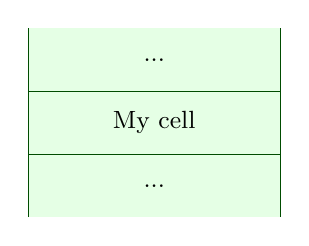
\begin{tikzpicture}[scale=0.8]
  \small
  \stacktop{}
  \cell{My cell}
  \stackbottom{}
\end{tikzpicture}

\section{Changing style}

{% tikzstyle will be local to this {...}
\tikzstyle{freecell}=[fill=blue!10,draw=blue!30!black]
\tikzstyle{occupiedcell}=[fill=blue!10!orange!10,draw=blue!30!black]
\tikzstyle{padding}=[fill=yellow!20,draw=blue!30!black]
\tikzstyle{highlight}=[draw=orange!50!black,text=orange!50!black]

\begin{drawstack}
  \cell{Uninteresting cell}
  \cell{Interesting cell} \cellround{Yes, this one!}
  \bcell{bcell}
  \padding{2}{Padding}
\end{drawstack}
}

\section{Example: Computing Factorial}

\begin{drawstack}[scale=0.8]
  \startframe
  \cell{N = 1}
  \cell{...}
  \finishframe{fact(1)}
  \startframe
  \cell{N = 2}
  \cell{...}
  \finishframe{fact(2)}
  \cell{$\vdots$}
  \startframe
  \cell{N = 5}
  \cell{...}
  \finishframe{fact(5)}
\end{drawstack}

\end{document}

%%% Local Variables:
%%% mode: latex
%%% TeX-master: t
%%% End:



	
	\section{Progettazione}
Il modulo partirà nell'elaborazione quando il segnale {\small\lstinline[columns=fixed]{i_start}} in ingresso verrà portato a 1.\newline
Il segnale \lstinline[columns=fixed]{i_start} rimarrà alto fino a che il segnale \lstinline[columns=fixed]{o_done} non verrà portato alto. Al termine della computazione (e una volta scritto il risultato in memoria), il modulo alza (cioè porta a 1) il segnale \lstinline[columns=fixed]{o_done} che notifica la fine dell'elaborazione. Se a questo punto viene rialzato il segnale \lstinline[columns=fixed]{i_start}, il modulo ripartirà con la fase di codifica.

\subsection{Scelte progettuali}
Si è scelto di descrivere il componente tramite una macchina a stati finiti (FSM).\newline
In VHDL sono stati utilizzati due process:

\begin{itemize}
	\item Un process per descrivere la parte sequenziale della FSM, ovvero, rappresentare i re-gistri di stato. Questo process si occupa anche di riportare la macchina nello stato di reset in corrispondenza del valore attivo del segnale \lstinline[columns=fixed]{i_rst}.
	
	\item Un process per descrivere la parte combinatoria della FSM, ovvero, determinare lo stato in cui evolve il sistema in funzione dei segnali in ingresso e dello stato corrente. 
\end{itemize}

In particolare il modulo confronta gli indirizzi ADDR e WZ sfruttando l'operazione di \textbf{sottrazione} e, nel caso di ADDR appartenente alla Working Zone, codifica la differenza (offset) in one-hot.\newline
La codifica one-hot è stata realizzata mediante l'uso di un registro inizializzato ad ogni avvio della FSM a "$0001$" e l'operazione di \textbf{shift} (a sinistra) di un numero pari alla differenza tra i due indirizzi.\newline
In aggiunta, si è preferito tenere memorizzate nel componente meno informazioni possibili. Ciò ha favorito un'occupazione d'area del modulo (in termini di flip-flop e look-up tables) molto piccola rispetto alla FPGA scelta inizialmente.\newline
Queste soluzioni offrono il \textbf{vantaggio di essere scalabili}, poiché se aumentasse il numero di working-zone da controllare, non sarebbe necessario aumentare di molto l'area del modulo solo per tenere memorizzati tutti gli indirizzi delle working-zone, nè reimplementare interamente parti del codice per supportare le ulteriori codifiche one-hot necessarie.\newline

Inoltre si è adottato un approccio che cercasse di:
\begin{itemize}
	\item ridurre il numero di transizioni effettuate per portare a termine la codifica dell'indirizzo;
	
	\item chiedere un dato alla RAM solo quando strettamente necessario, in modo da minimizzare gli accessi in memoria. Per esempio, una volta trovata la working-zone di appartenenza dell'indirizzo da codificare, risulta inutile un controllo delle eventuali working-zone rimanenti.
\end{itemize}
Il tutto si è tradotto in una progettazione della FSM con un numero di stati ridotto e in un attento utilizzo dei bus per comunicare con la RAM. 

\pagebreak

\subsection{Macchina a stati}
La macchina implementata (Figura \ref{fig:fsm_1}) è composta dai seguenti sei stati:

\begin{itemize}[itemsep=10pt]
	\item \texttt{IDLE}\newline
	Stato iniziale di reset in cui si attende che venga alzato il segnale \lstinline[columns=fixed]{i_start}. In caso di segnale \lstinline[columns=fixed]{i_rst='1'} si torna in questo stato.
	
	\item \texttt{FETCH\_ADDR}\newline 
	Stato in cui viene richiesto alla memoria l'indirizzo da codificare.
	
	\item \texttt{WAIT\_RAM}\newline
	Stato in cui si attende la risposta della memoria dopo una richiesta di lettura.
	
	\item \texttt{GET\_ADDR}\newline
	La prima volta (dopo un reset) che la macchina entra in questo stato viene memorizzato, in un apposito registro, l'indirizzo da codificare. Per risparmiare un periodo di clock, viene inoltre richiesto alla memoria l'indirizzo base della prima Working Zone (WZ 0).\newline
	Le successive volte viene richiesto l'indirizzo base della prossima Working Zone e viene letto dalla memoria l'indirizzo base della Working Zone richiesta precedentemente. Questo verrà confrontato direttamente con l'indirizzo da codificare per stabilirne l'eventuale appartenenza. In caso positivo, viene salvato l'offset in un registro e il sistema passa allo stato \texttt{WRITE\_BACK}.\newline
	Si torna in questo stato finché non si trova la Working Zone di appartenenza dell'indirizzo da codificare o fino a quando non si sono esaurite le Working Zone da controllare. 
	
	\item \texttt{WRITE\_BACK}\newline
	Stato in cui l'indirizzo codificato viene scritto nell'indirizzo 9 della memoria e si passa allo stato \texttt{DONE}.
		
	\item \texttt{DONE}\newline
	Stato finale in cui si pone il segnale \lstinline[columns=fixed]{o_done='1'}.\newline
	Si resta in questo stato fino a quando non si riceve \lstinline[columns=fixed]{i_start='0'} per poter poi abbassare il segnale \lstinline[columns=fixed]{o_done} e tornare nello stato \texttt{IDLE}.
\end{itemize}

\begin{figure}[!htb]
	%\setlength\abovecaptionskip{-5pt}
	
	\tikzset{
	loop above/.style={% original: above, in=75, out=105 loop
		above, in=75, out=105, loop,
		every loop/.append style={looseness=7}
	},
	loop right/.style={
		right, in=320, out=350, loop,
		every loop/.append style={looseness=7}
	}	
}

\begin{tikzpicture}[shorten >=1pt,font=\footnotesize,node distance=5cm,on grid,auto,
					initial text = {\lstinline[columns=fixed]{i_rst}='1'},
					state/.style={circle, draw, minimum size=2.5cm}] 
	\node[state,initial] (q_0)   {\texttt{IDLE}}; 
	\node[state] (q_1) [above right=of q_0] {\texttt{FETCH\_ADDR}}; 
	\node[state] (q_2) [right=of q_1] {\texttt{WAIT\_RAM}};
	\node[state] (q_3) [below=of q_2] {\texttt{GET\_ADDR}}; 
	\node[state](q_4) [below=of q_3] {\texttt{WRITE\_BACK}};
	\node[state](q_5) [left=of q_4] {\texttt{DONE}};
	
	\path[->] 
	(q_0) edge node {\lstinline[columns=fixed]{i_start}='1'} (q_1)
	      edge [loop right] node {\lstinline[columns=fixed]{i_start}='0'} ()
	(q_1) edge node {--} (q_2)
	(q_2) edge [bend left=45] node {--} (q_3)
	(q_3) edge [bend left=45] node [align=center] {"WZ non trovata"\\AND\\"altre WZ da analizzare"} (q_2)
	(q_3) edge node [align=center] {"WZ trovata"\\OR\\"finite WZ da analizzare"} (q_4)
	(q_4) edge node {--} (q_5)	  
	(q_5) edge [bend left] node {\lstinline[columns=fixed]{i_start}='0'} (q_0)
		  edge [loop above] node {\lstinline[columns=fixed]{i_start}='1'} ()
	;
\end{tikzpicture}
	\caption{rappresentazione della macchina a stati.}	
	\label{fig:fsm_1}
\end{figure}

	
	\section{Testing del componente}
Il corretto funzionamento del componente è stato verificato tramite l'utilizzo dei test bench. Tre sono le modalità di simulazione eseguite: \textit{Behavioural}, \textit{Post-Synthesis Functional} e \textit{Post-Synthesis Timing}.\newline
A partire dai test bench di esempio, sono stati costruiti altri test bench che cercassero di simulare il maggior numero di possibili scenari d'esecuzione del modulo.\newline
Di seguito sono riportati i casi di test più significativi. I primi due forzano il controllo di tutte le working-zone presenti in RAM.

\begin{enumerate}

	\item \textbf{WZ MISS}: l'indirizzo da codificare non appartiene a nessuna working-zone.
	\begin{figure}[!htb]
		\centering
		%\setlength{\belowcaptionskip}{-0.5cm}
		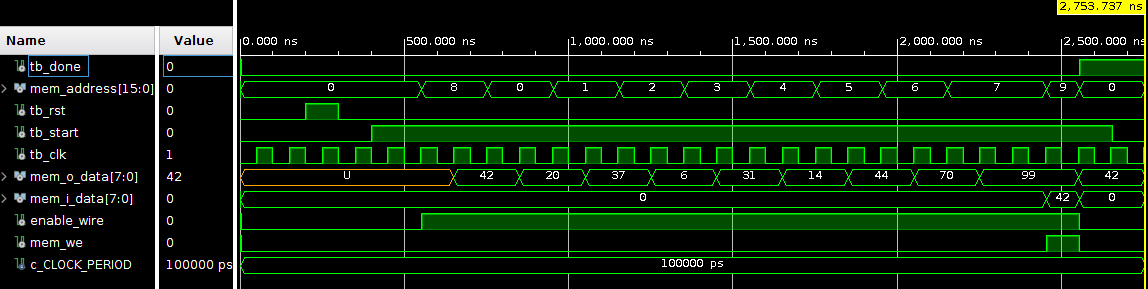
\includegraphics[scale=0.520]{images/wz_miss.png}
		\caption{waveform della simulazione con ADDR non appartenente a nessuna WZ.}
	\end{figure}
		
	\item \textbf{Ultima WZ HIT}: il test verifica la codifica dell'indirizzo nel caso in cui esso appartenga all'ultima working-zone disponibile in RAM (WZ 7).
	
	\item \textbf{Prima WZ HIT}: il test verifica la codifica dell'indirizzo nel caso in cui esso appartenga alla prima working-zone disponibile in RAM (WZ 0).
	\begin{figure}[!htb]
		%\setlength{\belowcaptionskip}{-0.5cm}
		\centering
		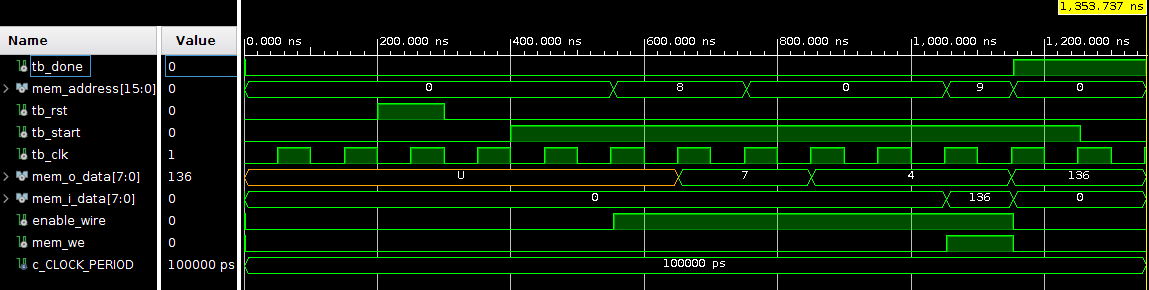
\includegraphics[scale=0.520]{images/first_wz_hit.png}
		\caption{waveform della simulazione con $ADDR=7$ appartenente alla prima WZ.}	
	\end{figure}

\end{enumerate}	

Ciascuno dei successivi test è stato eseguito sia in occorrenza \textit{\textbf{WZ MISS}} che \textit{\textbf{WZ HIT}}.

\begin{enumerate}[resume]
	
	\item \textbf{WZ adiacenti}: le working-zone caricate nella RAM sono una adiacente all'altra.
	
	\item \textbf{ADDR/WZ minimi}: l'indirizzo da codificare e/o una WZ corrispondono alla codifica in binario composta da soli zero "00000000" (0 in decimale).
	
	\item \textbf{ADDR massimo}: l'indirizzo da codificare corrisponde alla codifica in binario "01111111" (127 in decimale).
	
	\item \textbf{WZ massima}: l'indirizzo di una working-zone corrisponde alla codifica in binario "01111100" (124 in decimale). Questa rappresenta la massima codifica possibile su 8 bit (con il bit più significativo a 0) affinché la working-zone risulti completa, cioè con 4 indirizzi di offset (124, 125, 126, 127).

	\item \textbf{Reset asincrono}: il test verifica il comportamento della macchina quando il segnale di reset viene alzato in modo asincrono. La macchina torna nello stato di reset \texttt{IDLE} dove rimane in attesa di un nuovo segnale di inizio.
	\begin{figure}[!htb]
		\centering
		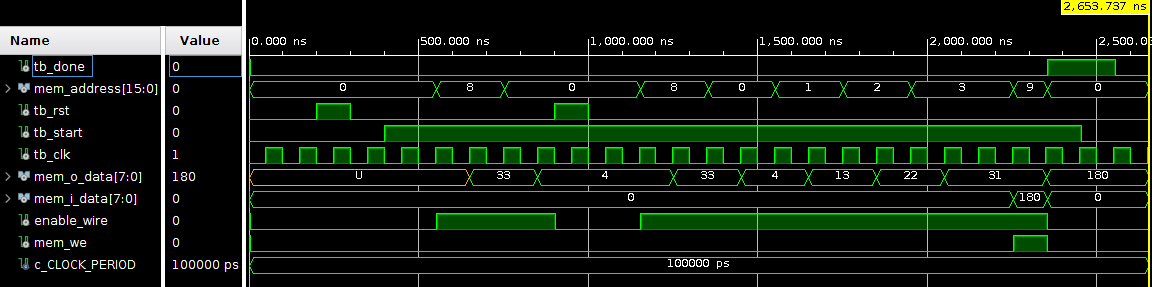
\includegraphics[scale=0.520]{images/async_reset.png}
		\caption{waveform della simulazione con reset asincrono.}	
	\end{figure}
	
	\item \textbf{Multi-start, stesse WZ}: il test effettua la codifica (in sequenza) di almeno due indirizzi diversi mantenendo invariate le working-zone durante ogni computazione.
	
	\item \textbf{Multi-start con reset (diverse WZ)}: il test effettua la codifica (in sequenza) di almeno due indirizzi. Le working-zone tra una computazione e l'altra vengono cambiate tramite l'asserzione del segnale \lstinline[columns=fixed]{i_rst}.
	
	\item \textbf{Frequenza elevata}: un caso di test è stato dedicato alla variazione della frequenza di elaborazione del modulo. Dal periodo di clock di default pari a 100ns si è testato fino ad un minimo di circa 5ns.
\end{enumerate}

Oltre ai test mirati proposti sopra, sfruttando la modalità batch di Vivado, sono stati si-mulati numerosi test bench generati casualmente da un apposito script scritto in Python.\newline

	
	\section{Risultati della sintesi}
Il componente è stato sintetizzato con successo. Di seguito vengono riportati alcuni dei risultati ottenuti durante questa fase.

\subsection{Registri sintetizzati}
In Tabella \ref{table:registers} sono elencati i registri sintetizzati.

\begin{table}[!htb]
	\centering
	\setlength{\belowcaptionskip}{-0.5cm}
	
	\begin{tabular}{ |c|c|l| }
		\hline
		\textbf{\# bit} & \textbf{Quantità} & \textbf{Descrizione} \\
		\hline
		16 & 1 & \specialcell{Indirizzo della RAM. \\ Si utilizzano 16 bit per semplificarne la gestione.} \\ \hline
		 8 & 2 & \specialcell{Indirizzo da codificare e indirizzo codificato in uscita. \\Vengono salvati per assicurare la corretta propagazione dei segnali.} \\ \hline
		 4 & 1 & \specialcell{Offset dell'indirizzo (${WZ}_{OFFSET}$).} \\ \hline
		 3 & 1 & \specialcell{Stato presente della macchina.\\ Sono necessari 3 bit per la codifica dei sei stati.} \\ \hline
		 1 & 5 & \specialcell{${WZ}_{BIT}$, segnale di controllo e tre segnali di uscita del componente.}\\
		\hline
	\end{tabular}

	\caption{}
	\label{table:registers}	
\end{table}

\subsection{Area utilizzata sulla FPGA}
Come da scelte progettuali, si è cercato di ridurre al minimo l'area occupata dal componente sulla FPGA target. Nell'ottica di realizzare componenti più complessi, si è ritenuto che questo encoder non dovesse richiedere risorse che andrebbero impiegate per altri scopi.\newline
Dal report fornito dallo strumento di sviluppo Vivado otteniamo le seguenti percentuali di area occupata rispetto alla FPGA target utilizzata.

\begin{table}[!htb]
	\centering
	\setlength{\belowcaptionskip}{-0.5cm}
	
	\begin{tabular}{ |c|c|c|c| }
		\hline
		\textbf{Tipo} & \textbf{Utilizzati} & \textbf{Disponibili} & \textbf{Percentuale} \\
		\hline
		FF & 32 & 269200 & 0.01\%\\ \hline
		LUT & 39 & 134600 & 0.03\%\\
		\hline
	\end{tabular}
	
	\caption{}
	\label{table:area}	
\end{table}


\subsection{Frequenza di funzionamento}
Con un calcolo approssimativo è possibile ottenere la massima frequenza a cui può operare il componente. Si consideri il periodo di clock $T_{clk}$ di $100 ns$ (da specifica). Dal report si ottiene un \textit{Worst Negative Slack} $WNS$ pari a $94.701 ns$. Il minimo periodo utilizzabile risulta:
\abovedisplayshortskip=5pt
\belowdisplayshortskip=8pt
\begin{equation*}
	T_{min} = T_{clk} - WNS = 100 ns - 94.701 ns = 5.299 ns
\end{equation*}


e quindi si ottiene la massima frequenza di funzionamento:

\abovedisplayshortskip=5pt
\belowdisplayshortskip=0pt
\begin{equation*}
	f_{max} = \frac{1}{T_{min}} = \frac{1}{5.299 ns} \approx 188.72 MHz.
\end{equation*}

	
	\section{Conclusione}
Il componente sviluppato simula correttamente un encoder di indirizzi secondo il metodo \textit{Working Zone}.\newline
La trasformazione della specifica in una macchina a stati finiti ha semplificato notevolmente la fase di architettura del modulo.\newline
Successivamente la macchina è stata trascritta in codice VHDL che è stato testato e sintetizzato correttamente.\newline
Infine, si è cercato di ottimizzare il codice (e quindi la macchina stessa) in modo da ridurre l'area occupata e abbattere i tempi d'esecuzione del modulo.

\end{document}
